% This is lnbip.tex the demonstration file of the LaTeX macro package for
% Lecture Notes in Business Information Processing from Springer-Verlag.
% It serves as a template for authors as well.
% version 1.0 for LaTeX2e
%
\documentclass[lnbip]{svmultln}
%
\usepackage{makeidx}  % allows for indexgeneration
\usepackage{graphicx}
% \makeindex          % be prepared for an author index
%
\newcommand{\mari}[1]{\footnote{MARI: #1}}
\begin{document}
%
\mainmatter              % start of the contribution
%
\title{Prototypes are forever\\
  Evolving from a prototype project\\ to a full-featured system}
%
\titlerunning{Prototypes are forever}  % abbreviated title (for running head)
%                                     also used for the TOC unless
%                                     \toctitle is used
%
\author{Hugo Corbucci\inst{1}, Mariana V. Bravo\inst{1}, Alexandre Freire da Silva\inst{1} and Paulo Morelli\inst{2}}
%
\authorrunning{Hugo Corbucci et al.}   % abbreviated author list (for running head)
%
%%%% list of authors for the TOC (use if author list has to be modified)
\tocauthor{Hugo Corbucci, Mariana V. Bravo, Alexandre Freire da Silva and Paulo Morelli}
%
\institute{Agilbits, Sao Paulo, Brazil,\\
\email{{hugo,marivb,freire}@agilbits.com.br}}

\maketitle              % typeset the title of the contribution
% \index{Ekeland, Ivar} % entries for the author index
% \index{Temam, Roger}  % of the whole volume
% \index{Dean, Jeffrey}

\begin{abstract}        % give a summary of your paper

%TODO Abstract
This paper shows our experience evolving a prototype to a full featured project.
%                         please supply keywords within your abstract

%TODO Keywords
\keywords {prototype, agile methods, }
\end{abstract}
%
\section{Introduction}

Prototyping is an activity that most developers have heard about. Fred
Brooks mentioned it in The Mythical Man-Month \cite{Brooks1975} as one
of the best ways to provide a quick view of a feature to the clients
or users to help them make a choice. Dynamic System Development Method
(DSDM)\cite{DSDM} is heavily based on prototyping and other agile
methods also adopt many ideas related to this concept like spykes\cite{XP} in the Extreme Programming exploration fase. 
However, those who have had some experience with this practice feel uncomfortable with it\cite{quem disse? esse tipo de afirmação é sempre bom ter uma citação, já apanhei bastante sobre isso. ale}.

Successful software prototypes look very much like complete features
given a certain execution path. Therefore it is common that the
customers are so satisfied that they want to integrate the
prototypes to the working system and move on. The problem is that
prototypes are frequently created in a ``quick and dirty'' fashion and
the result is not adequate to be incorporated in a full-featured
system. Yet it is quite hard to explain this fact to the stakeholders
who usually do not want to invest any more money in this ``already
working'' feature. The consequence is that they switch priorities and
 focus developer work efforts to other parts of the system and leave the rough
prototype lost within the code base. Months or years later, the
prototype becomes a part of the system but is filled with bugs,
unhandled corner cases and, frequently, crappy code. Nobody remembers
what it was supposed to do or whether it is really
important. Maintainability gets deeply affected and developers get
that natural and unpleasant I-told-you-so feeling. %TODO trauma?

Developers that have been through the pain of maintaining those dirty
prototypes are no longer enthusiastic to work with prototypes. If
they have to, they make it so that there will be absolutely no way to
integrate the prototype to the existing system by either using a
different platform, language or even creating prototypes in other
medias. That inflexibility can reduce the ability of responding to
changes quickly and therefore harm the clients' interests.

This paper presents how a four-people collocated team managed to start
a prototyping project and evolve it naturally to a full-featured
application. We have organized this experience report following the chronological order
of the project's evolution. Section \ref{sec:start} will present the
project as it was first introduced to the development team. Section
\ref{sec:working} presents the work process established by the team to
create the software based on prototypes.  After some time, the team
felt that the customer needed a full featured application, we describe this change in
 Section \ref{sec:changes}. The following section (Section
\ref{sec:adapting}) shows how the team adapted to change to
evolve the prototype to a production ready application. Finally Section \ref{sec:nowadays} presents the
current status of the project and the customer's feedback about it's evolution. Section \ref{sec:conclusion}
concludes with a summary of practices that were useful to pass through
this experience without much pain.

\section{Starting the project}
\label{sec:start}

Back in March 2008, our company was hired to do some consulting for
one of the largest movie producing companies in Brazil. The client had
a great idea for a software to write movie scripts but had absolutely
no knowledge about software development.  He wanted to mature the idea
and understand how much investment it would take to turn it into
working software in order to establish his business plan. The
company's job at the time was to scout the market, discover
competitors and provide an estimation of the work needed to develop
the client's idea.

For such work, one consultant was assigned to understand what were the
client's needs and desires and two developers were asked to analyze
the existing script writing programs and evaluate the possible
development paths. After about 3 weeks of consulting and studies, the
team handed a deck full of story cards with two estimates each, based
on the use of two possible platforms. The first platform was an
existing open source software with several features and a copy-left
license. The second one was an Eclipse Rich Client Application
developed from scratch using Eclipse's open source framework.

This initial estimation suggested that a four people team dedicating 4 daily work hours to the project
 would be able to build a working prototype of each feature described in about nine months of development using the
existing open source software and about one year using Eclipse's
platform. The open source solution had the advantage to provide full
functionality of several other features. For a complete system, the
estimation was well over 2 years of work on the Eclipse version and
about a year and a half for the open source one.

After some discussion, the client opted for the Eclipse based solution
due to the license restriction of the open source one which conflicted
with his business plan. He also chose to develop only a prototype of
the idea since 2 years seemed like a too heavy investment for him
alone.

After the exploration phase, the consulting contract ended and a new
negotiable scope contract\cite{tem citação pra esse tipo de contrato?} with emphasis on development effort was established. 
This new contract established a team of 4 developers working with open
scope that would be negotiated monthly, providing 160 hours of work each month. It specifically stated
that the developers would work on pairs all the time and that the
developed system should have automated tests for all the production code.

The project's goal was to create a high visual fidelity prototype with mostly faked or
simplified features and a few working ones. The client would use this
prototype to present his ideas to investors by October 2008. This
meeting would either boost the project's development to a full
featured system if the investors liked the idea or end its development
in case they rejected it.

That was the team's vision of the project when the development
begun. A short seven months project whose fate would be decided by its
capacity to impress investors. Therefore, the main goal was to provide
 support for the client's demonstration to ensure the
project's growth and success. The next section (Section
\ref{sec:working}) describes how the team organized itself to achieve
this goal.

\section{Prototyping phase}
\label{sec:working}

Given the project's objective, the customer was always prioritizing new features considering only one specific usage scenario. This meant that, for most features, there were several cases which the team was asked \textbf{not} to handle. Regarding the source code, this meant that no verification or validation was written and the prototype would crash if the user did not behave as expected. We also incorporated several spikes as permanent solutions and did not handle a fair amount of exceptions, ignoring errors.

The team knew since the beginning that the client would change his mind over time. After all, it was partly to better understand his idea and its applicability that he wanted to build this prototype. This meant that features would be developed to later be thrown away while code produced only for a quick spike was going to become part of the system. Therefore, since the beginning the team invested on design, automated tests and refactoring, just enough to keep the system flexible to receive the next changes. The team also made it clear for the client that he would need some work done on features after he accepted them in order to polish the work.

The first few iterations went quite smooth. The main features developed involved importing a script in a text-only format, providing a simple way to mark text with meta-data and a way to manipulate and visualize this data. For these first features, it was simple to avoid inconsistencies since there were not many business rules involved. Problems started to appear on later interations once we needed to save changes and handle script modifications with more complex business rules.

The client's demonstration script was evolving as the prototype did and the team had to use conditionals to ignore cases he would not enter in during his presentation to investors. By October 2008, the main features planned\mari{to sentindo falta de um paragrafo "classificando" as features que tinhamos no inicio, estilo o spreadsheet que o paulo mandou pra gente laaaa no inicio do projeto (ver email "Fwd: Story Touch projeto" do Ale) - vamos conversar - Ale: pode ser uma boa! explicar qual era o épico mais importante, que era a firula visual que ficou pronta aqui} were ready for demonstration, but not polished, the prototype provided high visual fidelity but lacked functionality fidelity. Even so, the client was not feeling completely confident to present the software to the investors because he had discovered and prioritized new features that he felt were important but that were still incipient in the prototype. However, he started to make contact with a few people to schedule a meeting by the end of November 2008 or start of December 2008. Those dates became our new deadline until which all efforts should be focused on making those incipient features available for the demonstration.

At this point, the pressure for polishing the new features increased since the project's fate would be decided at the demonstration and it was close! The customer wanted the team to ignore corner cases, speed up delivery and ensure the demonstration would run smoothly. The excitement from the important presentation to other people (only our one client and us had seen the software so far) was a strong motivation for the development team to deliver all features the client had asked for. Yet, despite unit testing and pair programming being mandatory rules on the team, the general will to quickly deliver the features decreased the code quality considerably.

Things were getting quite unpleasant from a development perspective but since the client satisfaction was still high, there was little that could be done. However, external interference was about to change the situation a bit. Section \ref{sec:changes} will explain how the project was affected and detail the new direction these changes pointed to.

\section{Changing the rules}
\label{sec:changes}

December 2008 arrived and passed without any meeting. The company that
the client was in contact with had just been acquired by another one
so any project presentation was useless until things settled
down. That news pushed the deadline away for another 3 or 4 months at
least. Along with this news came the information that the client had
formed a dramaturgy experts group to help him better understand how to
structure the application.

This new context relieved a 4 months pressure of upcoming deadline
over a team which was beginning to feel the burden of unhandled
technical debt. All members of the development team agreed that the
code was getting complex and the quality was decreasing which was
affecting productivity and speed. The software was now going to have a
set of beta testers and it needed to perform decently to allow the
users to suggest improvements in the work system.

The general feeling was that the project was no longer aimed at a
simple presentation to investors. It was softly switching to a more
elaborate end user oriented application. The current development
approach would not be able to support this new use of the system. The
change had to be clear to the client so that development efforts would
be directed to address this new way of working.

The warnings came quickly from the dramaturgy study group. They
started having trouble with several known and unknown corner cases,
unexpected behaviors and just plain old bugs. The client noticed this
 and decided it was time to invest more in usability and user experience. The
 team made it clear that this would also mean less new features delivered and even managed to dedicate a whole iteration to refactoring.

At this point, the client started to understand the dilemma that the
developers had felt so far. How to keep a good rhythm of new feature delivery
and still cover most use cases of existing features? Another critical
issue in the software was that, so far, most features were aimed at
visualization and insertion of meta data in the scripts, but users
were claiming for basic text editing features that had been ignored so far.

The team estimated that to have an editor with the basic functionality
expected by the client would take at least three full iterations. This
was not welcomed by the client since it would mean that no new
features would be added until the moment when he would possibly be able to show the
software to investors. So he took another action which indicated
changes in the business plan of the project. The development team suggested that another team could work on text editing features parallel to them so that they could continue working on the new features he wanted.

After some research we discovered an open source
Eclipse Rich Client WYSIWYG (What You See Is What You Get) HTML
editor\footnote{\url{http://onpositive.com/richtext/} - Last accessed on
20/02/2010}. The editor relied on a reimplementation of Eclipse's
StyledText component which is responsible for rendering text within
Eclipse editors. This component was close enough from the one we
needed to implement, having some of the functionality our client wanted on our
application. So the client outsourced the development of this
underlying infra-structure to this open source project as a way to keep the new-feature delivery
velocity while attending the users' requests.

Meanwhile, the development team was concerned with the increasing
complexity so they started to track some data from the source
code. The first metrics was the amount of \texttt{FIXME},
\texttt{TODO} and \texttt{XXX} marks in the code. As previously
mentioned, the development team added those marks everywhere the felt
a corner case or a behavior existed but was not handled. Each mark had
a small comment associated and the kind of the mark determined the
criticality of the problem. Figure \ref{fig:TODOs} shows the evolution
of those marks during the project. Notice that the first data
collection of those marks is dated for mid July 2009.

\begin{figure}[hbt]
  \centerline{
    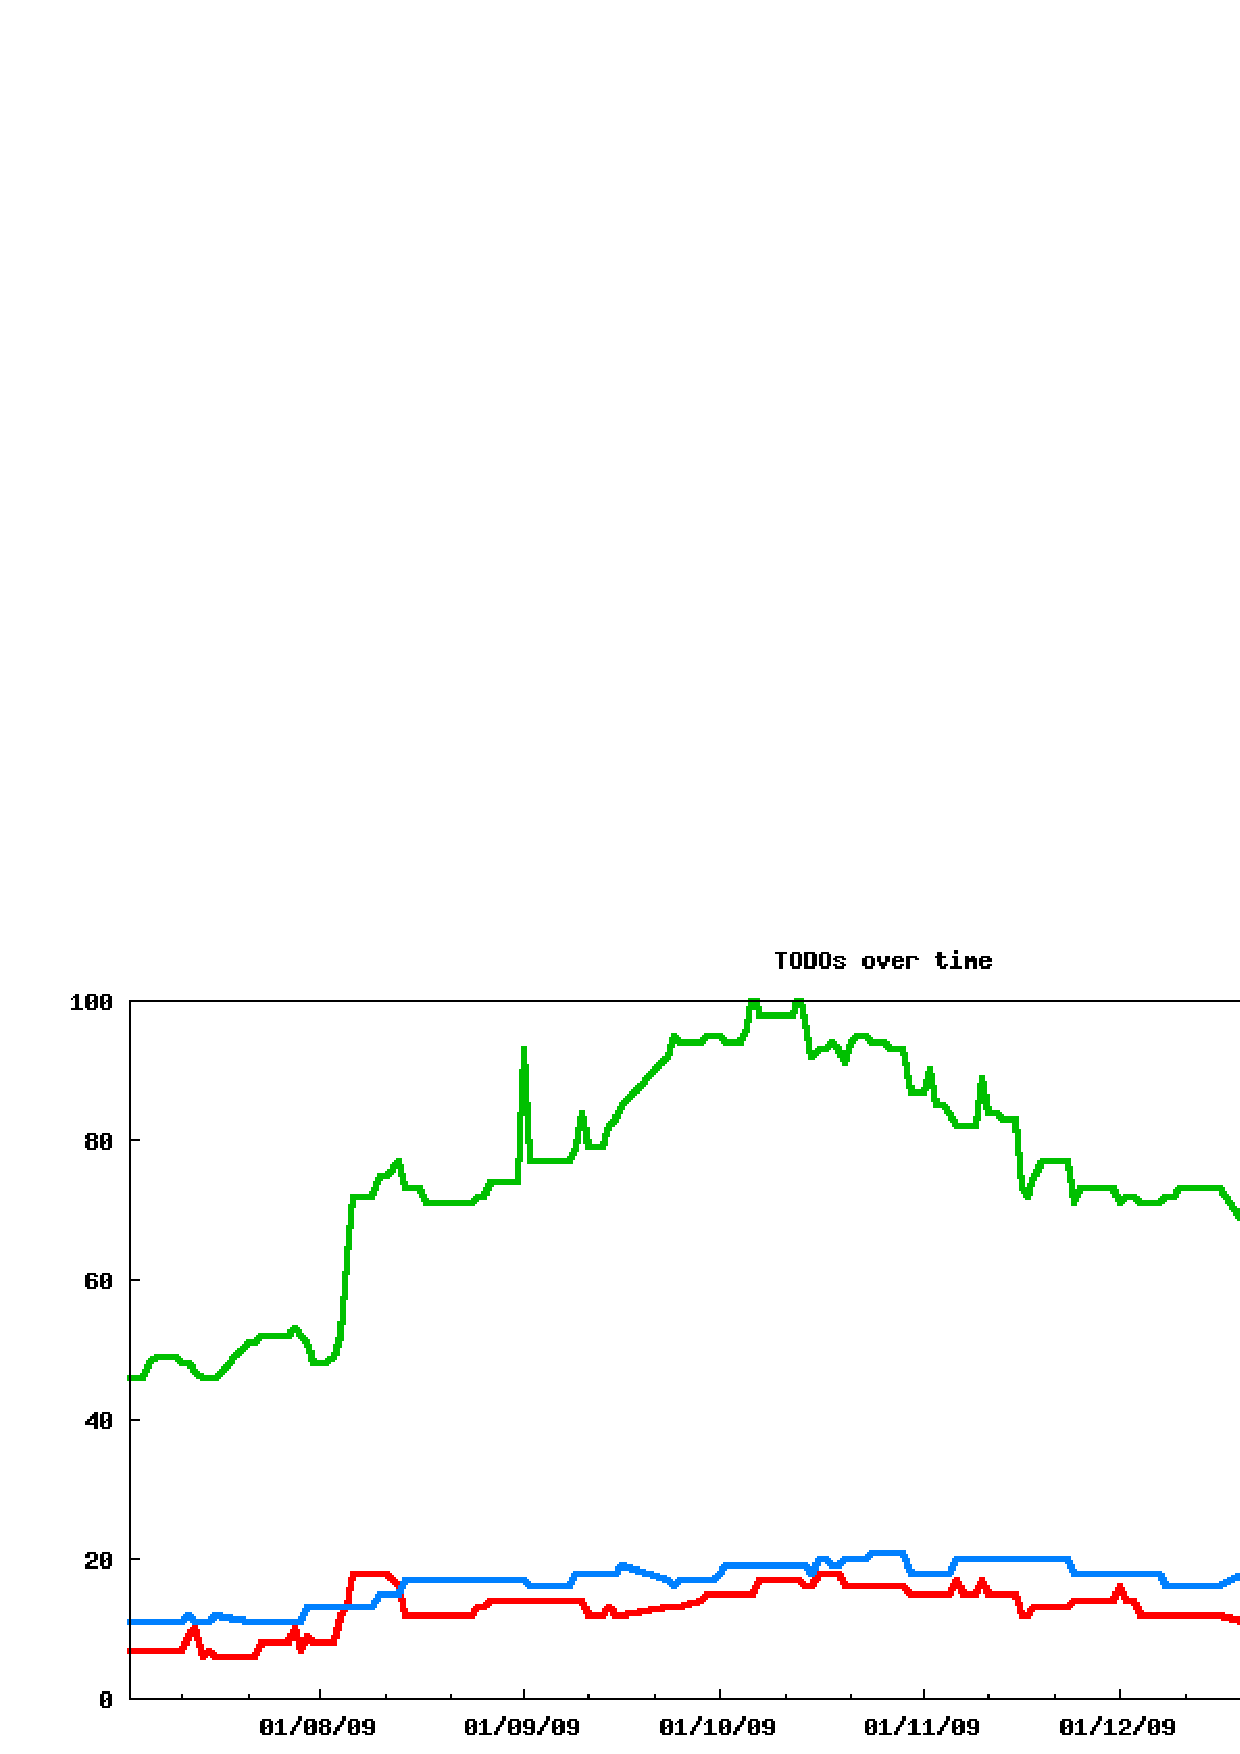
\includegraphics[width=120mm]{TODOs.png}
  }
  \caption{Evolution of FIXME, TODO and XXX marks in the source code}
  \label{fig:TODOs}
\end{figure}

\begin{figure}[hbt]
  \centerline{
    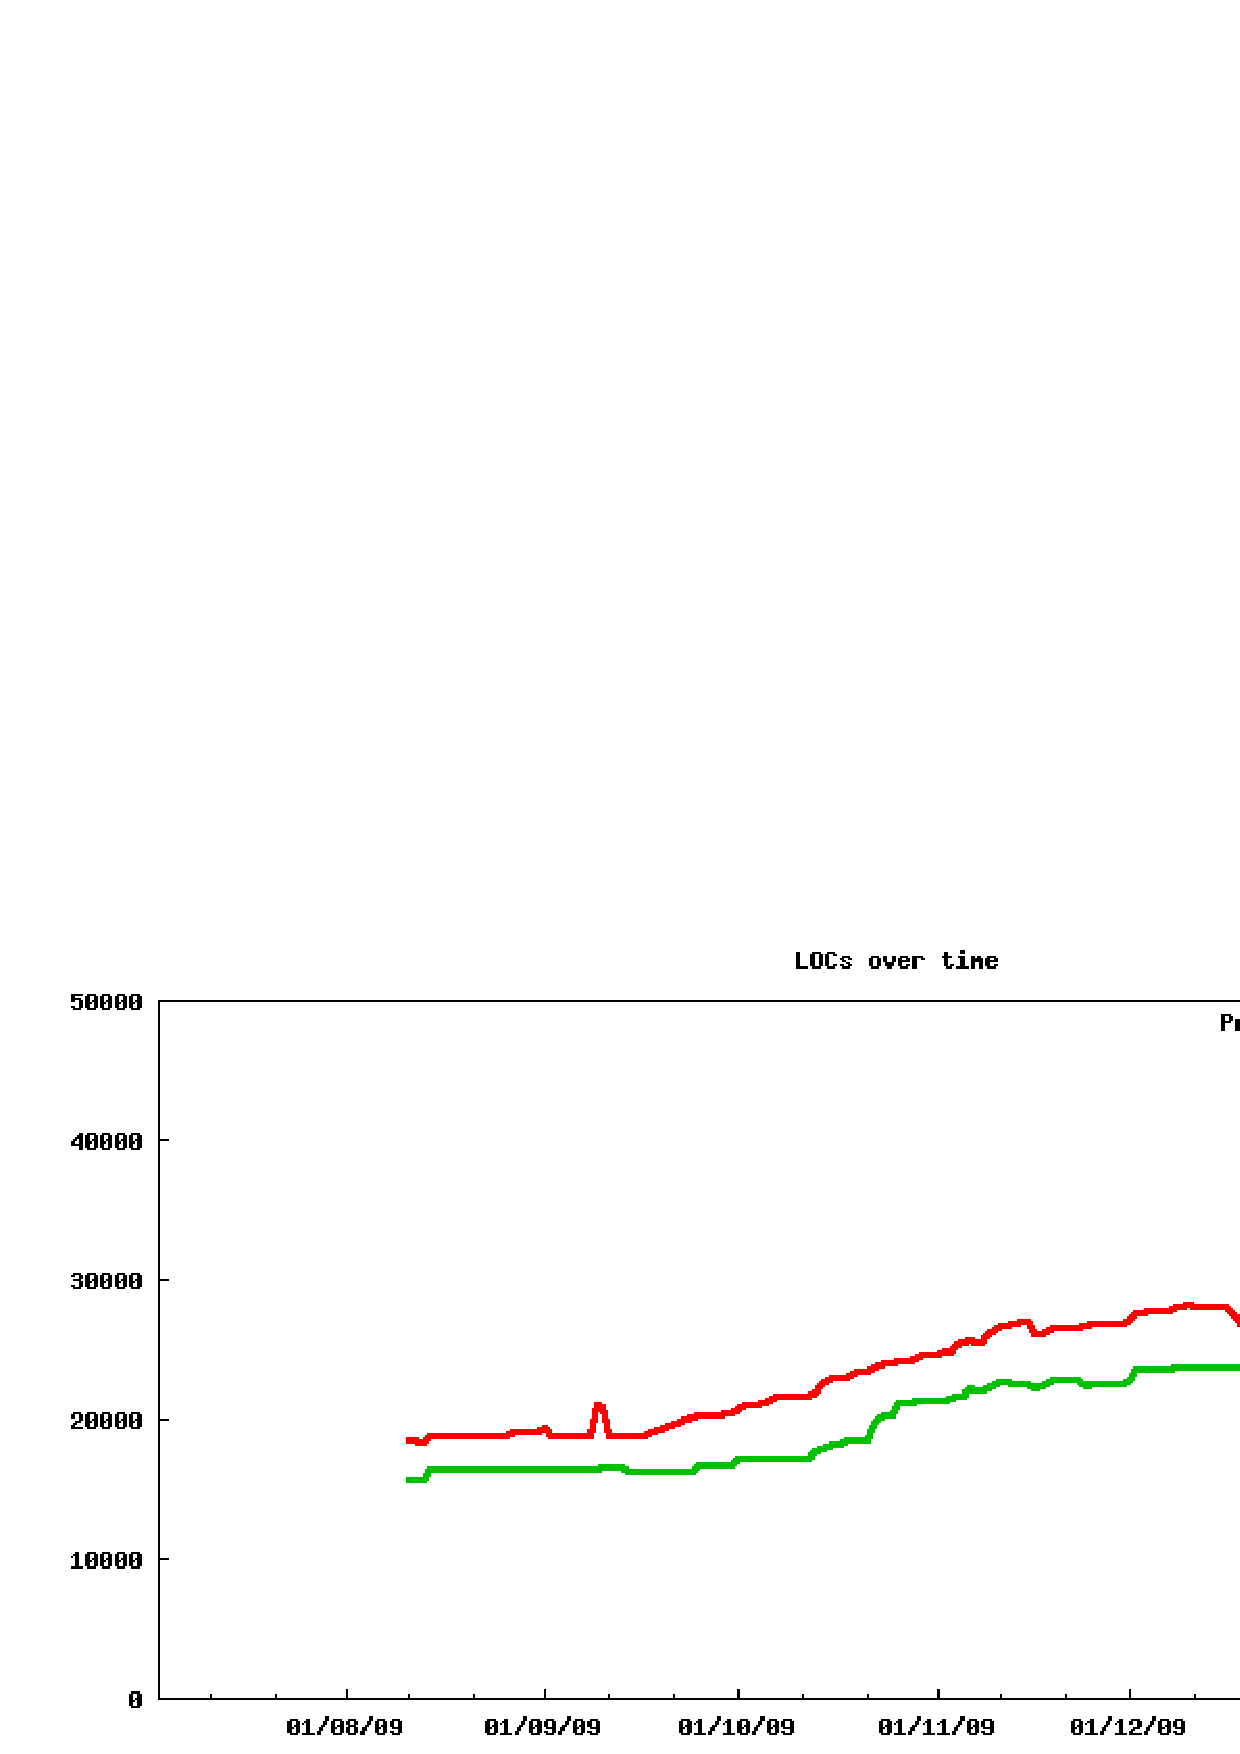
\includegraphics[width=120mm]{LOCs.png}
  }
  \caption{Evolution of production }
  \label{fig:LOCs}
\end{figure}

\begin{figure}[hbt]
  \centerline{
    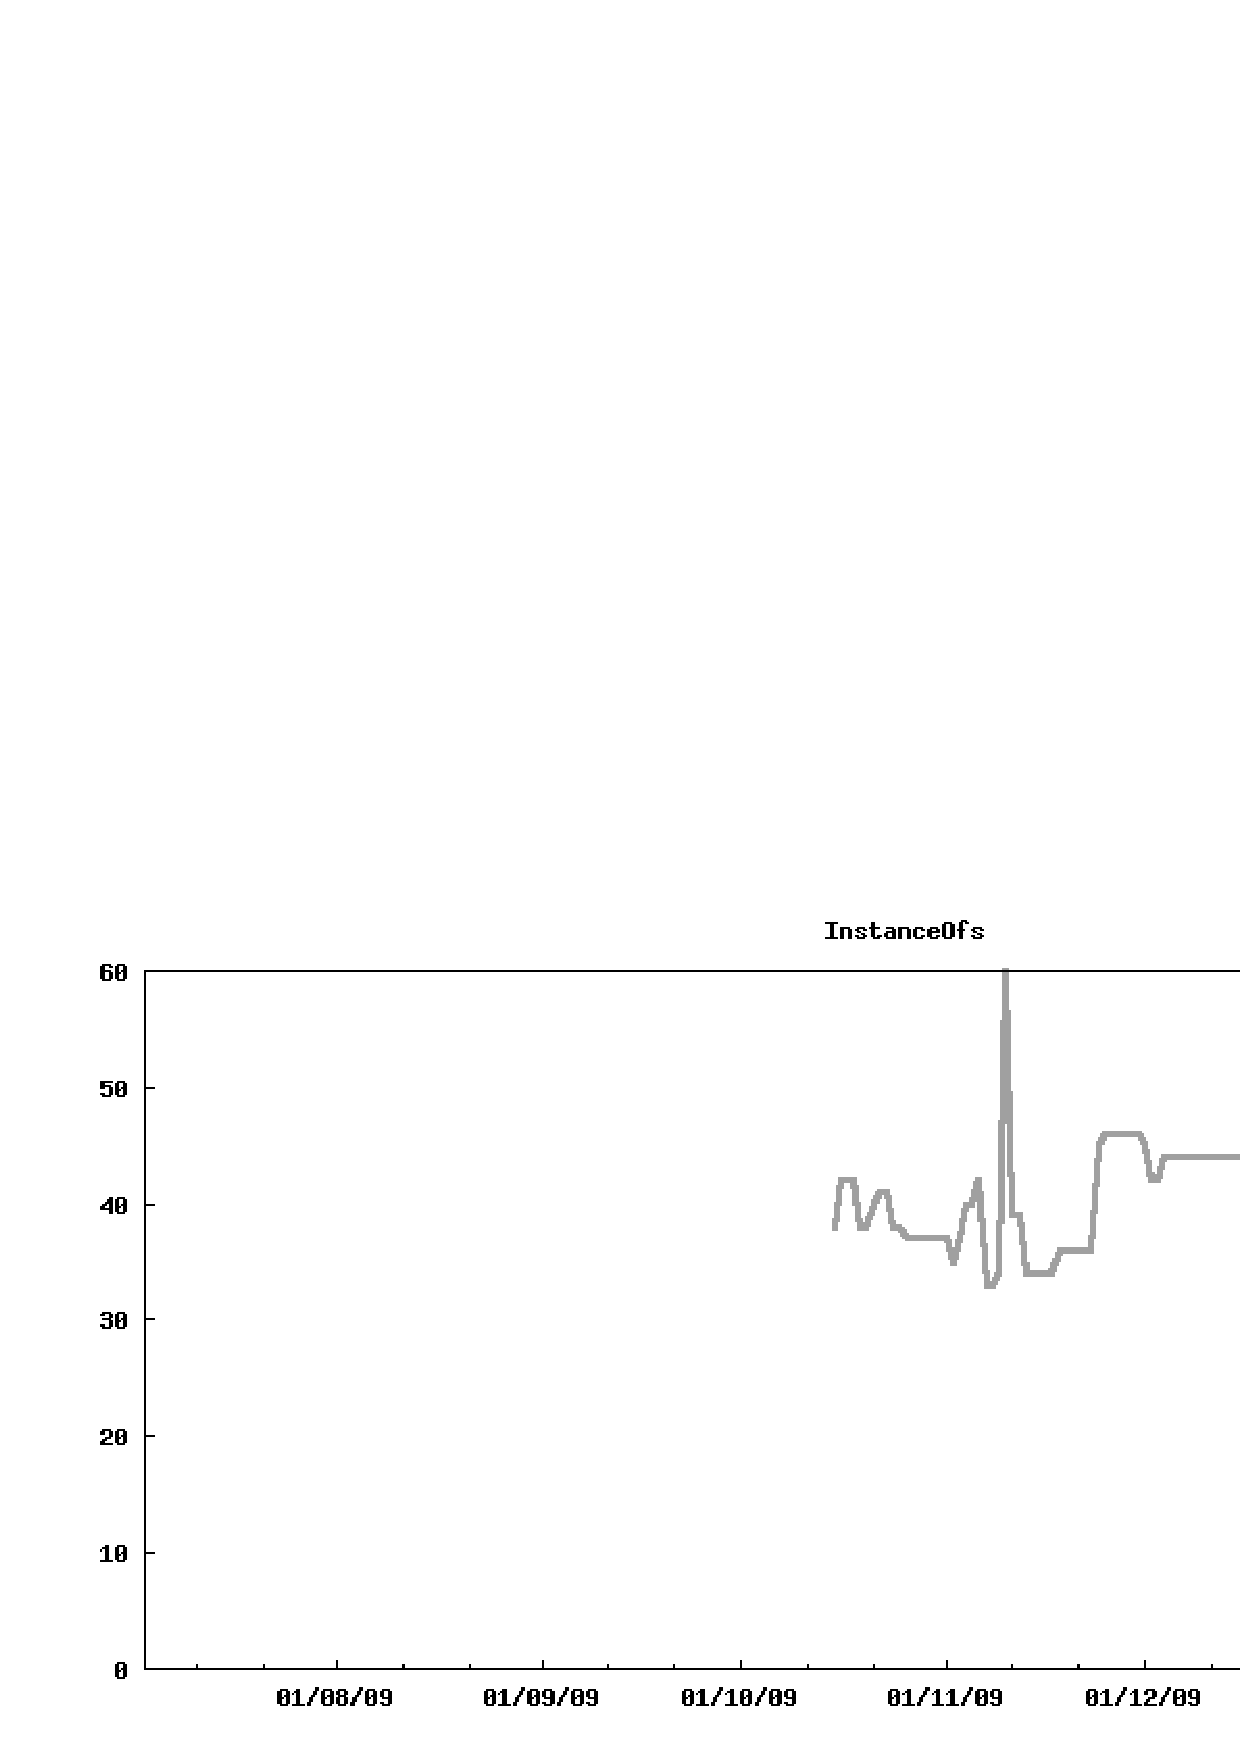
\includegraphics[width=120mm]{InstanceOfs.png}
  }
  \caption{Evolution of instanceof in the code }
  \label{fig:InstanceOfs}
\end{figure}

\begin{figure}[hbt]
  \centerline{
    \includegraphics[width=120mm]{refactoring.png}
  }
  \caption{Explicit refactoring time by iteration - acho que se esse gráfico também fosse por data seria melhor pq dava pra comparar com os outros. ale}
  \label{fig:refactoring}
\end{figure}

\section{Adapting to the new rules}
\label{sec:adapting}

Investing in reducing instanceof uses, TODOs and FIXMEs as well as
increasing line of tests. Noticing most issues are coming from
UI. SWTBot?

Effort dedication to integrate the new outsourced component developed.

Always handle (even if it means throwing an error to the log) corners
cases or unexpected input/paths. Always refactor before completing any
task. Tolerance 0 to bugs. Bug means highest priority.

Help the customer understand inconsistencies with his business model and rules, evolve and adapt existing features to be more consistent.

Introducing another developer in the team.

\section{Current status and customer feedback}
\label{sec:nowadays}

Test coverage

Testing in other platforms

Merciless decoupling

\begin{enumerate}
\item Before beginning the project, what were your expectations? How did you imagine the software you wanted and what it would become?
\item How did your idea evolve during the project? What took you to change your plan?
\item What effect had the fact that you could test your higher priority ideas with working software being delivered often?
\item What do you think about the application you have today in relationship to what you expected in the begining?
\item How do you evaluate the interactive learning process?
\item How do you evaluate the development process?
\item How satisfied are you with the evolution of the application?
\end{enumerate}

\section{Conclusion}
\label{sec:conclusion}

Team's effort to keep tests level (ignoring known issues not solved).

Refactor tests.

Refactor prototypes (their code must be good).



%
% ---- Bibliography ----
%
\begin{thebibliography}{5}

\bibitem{Brooks1975} Brooks Jr., F.P.: The Mythical Man Month: Essays
  on Software Engineering. Addison-Wesley (1975)


%ale: achei que era uma boa ter mais referências sobre prototipos. eu tirei essa história de prototipos de alta fidelidade visual ou alta fidelidade funcional de uma apresentação que vi sobre UX e prototipagem de interface lá na locaweb, no scholar.google achei isso aqui:

% http://74.125.155.132/scholar?q=cache:ezGZKBBRVhwJ:scholar.google.com/+software+prototype&hl=pt-BR&as_sdt=2000

% e http://www.imamu.edu.sa/Scientific_selections/abstracts/Documents/A%20Systematic%20Look%20At%20Prototyping.pdf

\end{thebibliography}
%
\end{document}
